\section{Data Logic Layer}

\subsection{Entity-Relationship Schema}

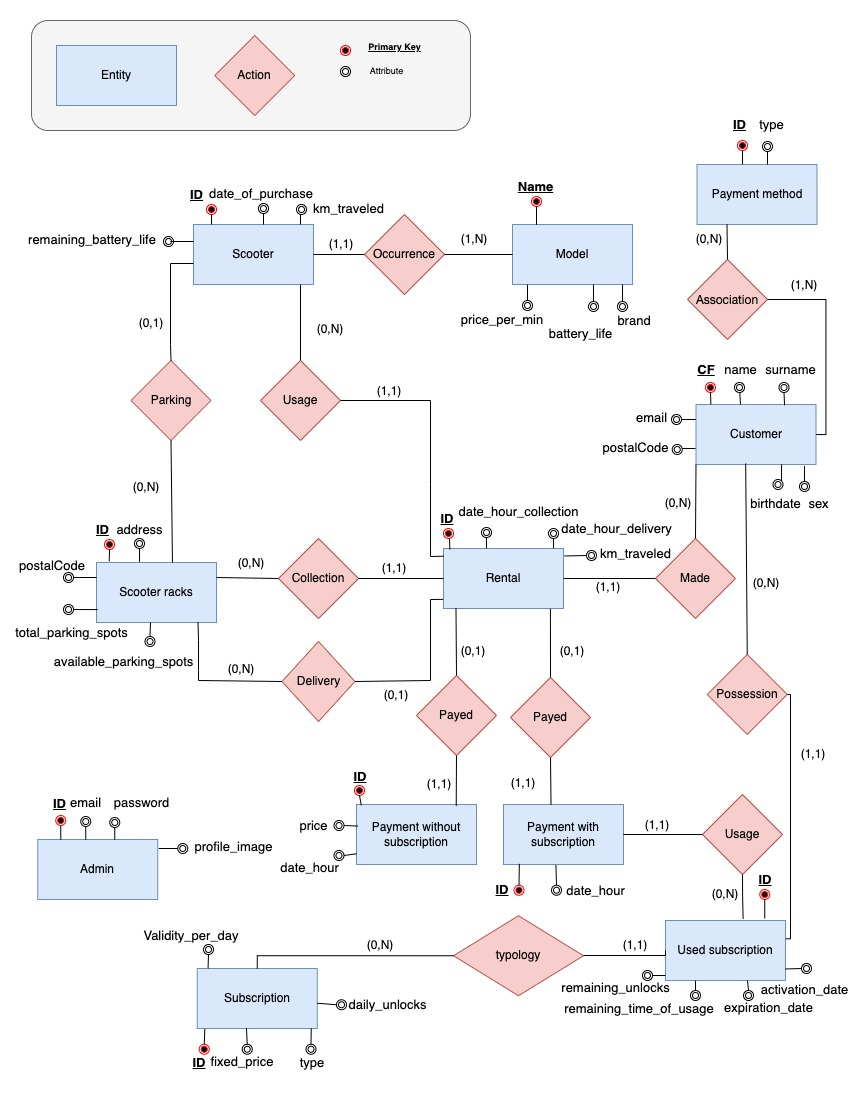
\includegraphics[scale=0.52]{sections/DLL/Wascoot_Final_ER_Chema-Page-1.jpg}

%Describe here your ER schema



\subsection{Data Dictionary: Entity Table}

\begin{longtable}{|p{.20\columnwidth}|p{.2\columnwidth} |p{.5\columnwidth}|p{.1\columnwidth} |} 
\hline
\textbf{Entity} & \textbf{Description} & \textbf{Attributes} & \textbf{P.Key}  \\\hline

Model & Entity representing the various models of a scooter. & 
\begin{itemize}
    \vspace{-1em}
    \item \textbf{Name}; specific type or version of the scooter;
    \item \textbf{Price per min}; The amount of money for renting scooter for a minute;
    \item \textbf{Brand}: model's manufacturer/company;
    \item \textbf{Battery life}: model's battery life.
\end{itemize} & Name \\\hline                 

Scooter &  This entity represents the specific scooter. A number of scooters are provided for renters. & 
\begin{itemize}
    \vspace{-1em}
    \item \textbf{ID}: scooter identifier; 
    \item \textbf{Date of purchase}: when scooter has been bought;
    \item \textbf{Km traveled}: distance covered by the scooter;
    \item \textbf{Remaining battery life}: how much of the original battery life is left.
\end{itemize} & ID \\\hline

Scooter racks & Structures designed to store and secure scooters when not in use. & 
\begin{itemize}
    \vspace{-1em}
    \item \textbf{ID}: scooter rack identifier;
    \item \textbf{Address}: address of the parking spot;
    \item \textbf{Postal code}: postal code of the rack's area; 
    \item \textbf{Total parking spots}: parking spot in this scooter rack; 
    \item \textbf{Available parking spots}: unoccupied parking spots in this scooter rack. 
 \end{itemize} & ID \\\hline


Rental & This entity represents the process of renting a scooter. & 
\begin{itemize}
    \vspace{-1em}
    \item \textbf{ID}: id of a specific scooter rental transaction;
    \item \textbf{Date and hour collection}: date and hour in which a scooter is rented;
    \item \textbf{Date and hour delivery}: date and hour in which a scooter is returned  and delivered;
    \item \textbf{Km traveled}: km traveled by the customer with this rental.
 \end{itemize} & ID \\\hline

Customer & People registered in the application that can rent a scooter. & 
\begin{itemize}
    \vspace{-1em}
    \item \textbf{CF}: fiscal code of the customer;
    \item \textbf{Email}; Email address of customer;
    \item \textbf{Name}; The name of customer;
    \item \textbf{Surname}; The surname of customer;
    \item \textbf{Postal code}; The address of postal of customer;
    \item \textbf{Sex}: customer's gender;
    \item \textbf{Birthdate}: date when the customer was born on. 
\end{itemize} & CF \\\hline

Admin & Entity representing the information regarding application's admins. & 
\begin{itemize}
    \vspace{-1em}
    \item \textbf{ID}; Admin identifier; 
    \item \textbf{Profile image}: admin's profile picture;
    \item \textbf{Email}; The email address of admin
    \item \textbf{Password}. Secret access to admin; 
\end{itemize} & ID \\\hline

Payment Method & Entity that lists the various types of payment methods. & 
\begin{itemize}
    \vspace{-1em}
    \item \textbf{ID}; Payment methods identifier; 
    \item \textbf{Type}: name of the payment method.
\end{itemize} & ID \\\hline

Payment without Subscription & Entity representing the one time payments. & 
\begin{itemize}
    \vspace{-1em}
    \item \textbf{ID}; The one-time payment identifier; 
    \item \textbf{Price}: price payed at the checkout after using the scooter;
    \item \textbf{Date and hour}: when the payment has been received.
\end{itemize}
& ID \\\hline

Payment with Subscription &  Entity representing payments &
\begin{itemize}
    \vspace{-1em}
    \item \textbf{ID}; Payment identifier;
    \item \textbf{Date and hour}: when the subscription's payment has been received.
\end{itemize}
& ID \\\hline

Used Subscription & & 
\begin{itemize}
    \vspace{-1em}
    \item \textbf{ID}; Usage identifier;
    \item \textbf{Remaining time of usage}: how much time until the subscription ends;
    \item \textbf{Activation date}: when the subscription started;
    \item \textbf{Expiration date}: when the subscription ends;
    \item \textbf{Remaining unlocks}: how many other times can the customer unlock a scooter today.
\end{itemize}
& ID \\\hline

Subscription & & 
\begin{itemize}
    \vspace{-1em}
    \item \textbf{ID}; Subscription identifier;
    \item \textbf{Fixed Price}: price of this subscription;
    \item \textbf{Type}: subscriptions' types differ based on how many days it covers (examples: 1day, 30days, 6months, ...) 
    \item \textbf{Daily Unlocks}: how many times can the customer unlock scooters in a day with this subscription.
    \item \textbf{Validity per Day}: how many hours can the customer use scooters with this subscription.
\end{itemize}
& ID \\\hline

\end{longtable}





